% ============================================================
%  RBAC-HNSW: Access-Controlled Vector Search
%  BioDMS @ VLDB 2026 — Project Talk Submission (4 pages)
%
%  Format: acmart sigconf (PVLDB Volume 19 style)
%  Compile: pdflatex → bibtex → pdflatex × 2
% ============================================================
\documentclass[sigconf,nonacm]{acmart}

\settopmatter{printacmref=false}
\renewcommand\footnotetextcopyrightpermission[1]{}
\pagestyle{plain}

% ── Packages ──────────────────────────────────────────────────────────────────
\usepackage{microtype}
\usepackage{booktabs}
\usepackage{enumitem}
\usepackage{algorithm}
\usepackage{algpseudocode}
\usepackage{graphicx}
\usepackage{xcolor}
\usepackage{url}
\usepackage{balance}
\usepackage{hyperref}
\hypersetup{colorlinks=true,linkcolor=blue!70!black,
            citecolor=blue!70!black,urlcolor=blue!70!black}

% ── Title & authors ───────────────────────────────────────────────────────────
\title{RBAC-HNSW: Access-Controlled Approximate Nearest-Neighbor Search\\
       for HIPAA-Governed Clinical Embeddings}

\author{Brendan Loalt}
\affiliation{%
  \institution{Independent Researcher}
  \city{}\country{USA}}
\email{brendanloalt@gmail.com}

% ── Document ──────────────────────────────────────────────────────────────────
\begin{document}

% Abstract must precede \maketitle in acmart
% ── Section: Abstract ────────────────────────────────────────────────────────
\begin{abstract}
Modern clinical AI systems store millions of high-dimensional vector
embeddings of patient records and must answer similarity search queries
in real time---while strictly enforcing fine-grained access control
policies mandated by regulations such as HIPAA.
Today, no vector database index handles this requirement efficiently
across the full spectrum of \emph{query selectivity}: the fraction of the
database a given user is permitted to see.
Post-filtering (retrieve candidates, then discard unauthorized results)
collapses to near-zero recall when access is restricted to $\leq 1\%$
of records.
Brute-force pre-filtering achieves exact results but degrades to
single-digit queries per second at broad access levels.
Multi-index architectures consume 8--64$\times$ more memory for realistic
role hierarchies.

We present \textbf{RBAC-HNSW}: a single modification to the
Hierarchical Navigable Small World (HNSW) graph-search algorithm that
enforces Role-Based Access Control (RBAC) at the node level, before the
expensive distance computation, while \emph{routing through} denied nodes
to preserve graph connectivity.
A 64-bit bitmask co-located with each vector adds only 0.24\% memory
overhead and costs $\approx\!1$ CPU cycle per access check.
On a 50{,}000-vector synthetic clinical dataset (BioBERT-scale,
768-dimensional), RBAC-HNSW achieves $\geq 0.90$ recall@10 across all
tested selectivity levels (0.02\%--40\%) and adds negligible memory
compared with the best multi-index competitor.
This paper presents the algorithm, a realistic HIPAA-motivated bitmask
schema for hospital access hierarchies, and an empirical evaluation
targeting the data-management community.
\end{abstract}


\begin{CCSXML}
<ccs2012>
 <concept>
  <concept_id>10002951.10002952.10003190</concept_id>
  <concept_desc>Information systems~Database query processing</concept_desc>
  <concept_significance>500</concept_significance>
 </concept>
 <concept>
  <concept_id>10002951.10002952.10002953.10010820.10003208</concept_id>
  <concept_desc>Information systems~Data privacy</concept_desc>
  <concept_significance>300</concept_significance>
 </concept>
</ccs2012>
\end{CCSXML}
\ccsdesc[500]{Information systems~Database query processing}
\ccsdesc[300]{Information systems~Data privacy}

\keywords{approximate nearest-neighbor search; HNSW; role-based access control;
          vector database; clinical informatics; HIPAA; similarity search}

\maketitle

% ── Main sections ─────────────────────────────────────────────────────────────
% ── Section: Introduction ─────────────────────────────────────────────────────
\section{Introduction}
\label{sec:intro}

The deployment of transformer-based language models in clinical medicine
has produced a new class of infrastructure challenge: \emph{access-controlled
approximate nearest-neighbor (ANN) search} over protected health information
(PHI).
Consider a hospital AI system that helps clinicians find similar past cases.
The system stores BioBERT~\cite{lee2020biobert} embeddings of one million
clinical notes (768-dimensional float vectors) and must answer each query
in under 10 milliseconds.
Crucially, every query result must satisfy the Health Insurance Portability
and Accountability Act (HIPAA): an Oncology physician must not see Psychiatry
notes; a researcher may access only records with explicit consent for their
specific study.

\smallskip
\noindent\textbf{The selectivity problem.}
In Role-Based Access Control (RBAC)~\cite{ferraiolo2001proposed}, each user
holds a \emph{permission mask} that determines which records they may read.
The \emph{selectivity} of a query is the fraction of the database accessible
to the querying user.
In a realistic hospital, selectivity varies from $\approx\!80\%$ (senior
administrator with broad access) down to $\approx\!0.1\%$ (researcher querying
genomic data from HIV-positive trial participants).
No existing ANN index handles this full range efficiently:

\begin{itemize}[leftmargin=1.4em,itemsep=1pt,topsep=2pt]
  \item \textbf{Post-filtering.}
    Standard HNSW retrieves a candidate set and filters by access mask.
    At 0.1\% selectivity, only $\approx\!1{,}000$ of $1{,}000{,}000$ records
    are accessible; a beam of width $\mathit{ef}\!=\!200$ explores far too
    few nodes to reach 10 accessible results reliably---recall collapses
    toward zero~\cite{malkov2020efficient}.

  \item \textbf{Pre-filtering (brute-force).}
    Build the accessible subset on-the-fly and scan it exhaustively.
    Exact results, but $O(|\text{accessible}| \times d)$ work per query:
    at 40\% selectivity over one million vectors, this reduces throughput
    to single-digit queries per second (QPS)~\cite{gollapudi2023filtered}.

  \item \textbf{Multi-index architectures (e.g., SIEVE~\cite{zhang2025sieve}).}
    Maintain one HNSW index per role.
    Good recall and throughput, but memory scales with $|\text{roles}|$:
    64 roles $\Rightarrow$ 64$\times$ the baseline index footprint
    ($\approx\!213$~GB for one million 768-dim vectors; Section~\ref{sec:eval}).
\end{itemize}

\smallskip
\noindent\textbf{Our contribution: RBAC-HNSW.}
We present a \emph{single algorithmic modification} to the HNSW greedy
search that gates on a 64-bit bitmask before computing the vector distance.
Denied nodes are not pruned from graph traversal---their neighbor lists are
still used to \emph{route} the beam toward accessible regions---preventing
the ``connectivity deserts'' that cause post-filtering recall to collapse.

Concretely, the access check
$(\mathit{node\_mask} \;\&\; \mathit{query\_mask}) = \mathit{query\_mask}$
costs one CPU instruction ($\approx\!1$~ns) and is evaluated before the
$768$-multiply cosine distance ($\approx\!30$~ns).
The mask is stored inline with each HNSW node pointer, fitting both in a
single 64-byte CPU cache line~\cite{drepper2007every}.
Memory overhead: $8$~bytes per vector $=$ \textbf{0.24\%} above vanilla HNSW.

\smallskip
\noindent\textbf{Scope of this paper.}
This work targets the \emph{data management community}, framing access-controlled
vector search as a database systems problem.
We present the algorithm (Section~\ref{sec:algorithm}), a biologically motivated
evaluation dataset (Section~\ref{sec:dataset}), and empirical results across
five selectivity levels (Section~\ref{sec:eval}).
Our open-source implementation is available at
\url{https://github.com/patriotsbreeze/Similarity-RBAC}.

% ── Section: Algorithm ───────────────────────────────────────────────────────
\section{The RBAC-HNSW Algorithm}
\label{sec:algorithm}

\subsection{Bitmask Encoding}
\label{sec:bitmask}

Each vector $v$ is assigned a 64-bit unsigned integer $v_m$ encoding its
access requirements.
A query with permission mask $q_m$ may access $v$ if and only if:
\[
  (v_m \;\mathbin{\&}\; q_m) = q_m
\]
That is, the node must possess \emph{at least} every permission bit required
by the query.
This subsumes standard RBAC role-hierarchy checks: if role $R_1$ inherits
from $R_2$, set all $R_2$-bits inside $R_1$'s mask.
Figure~\ref{fig:rbac_schema} shows the 64-bit layout used in our clinical
benchmark (see Section~\ref{sec:dataset}).

The mask is stored adjacent to the node's vector pointer in memory, so a
single 64-byte cache-line fetch~\cite{drepper2007every} delivers both fields.
The bitwise AND and comparison together constitute one CPU instruction
($\approx\!1$~ns), evaluated \emph{before} the distance computation
($\approx\!30$~ns for 768-dim cosine similarity).

\subsection{Two-Gate Greedy Search}
\label{sec:search}

Algorithm~\ref{alg:rbac_search} presents the modified HNSW layer-0 search.
The key departure from vanilla HNSW is in lines~\ref{alg:gate1}--\ref{alg:route}:
when a neighbor node $n$ fails the RBAC gate, we \emph{do not discard it}.
Instead, we add $n$ to the routing frontier so its own neighbor list can
direct the beam toward accessible regions.
Distance is only computed (line~\ref{alg:gate2}) when the access check passes.

\begin{algorithm}[t]
\small
\caption{RBAC-HNSW Greedy Search (Layer 0)}
\label{alg:rbac_search}
\begin{algorithmic}[1]
\Require Graph $G$, query $\mathbf{q}$, query mask $q_m$, result count $k$, beam $\mathit{ef}$
\Ensure Top-$k$ accessible nearest neighbors
\State $\mathit{results} \leftarrow$ min-heap; $\mathit{routing} \leftarrow$ priority queue; $\mathit{visited} \leftarrow \emptyset$
\State $e \leftarrow \textsc{EntryPoint}(G)$; $\mathit{visited} \leftarrow \{e\}$
\If{$\textsc{RBACCheck}(e, q_m)$} \Comment{Gate 1}
    \State push $(\textsc{Dist}(\mathbf{q}, e),\, e)$ into $\mathit{results}$ and $\mathit{routing}$
\Else
    \State push $(\infty,\, e)$ into $\mathit{routing}$ \Comment{Route through denied}
\EndIf
\While{$\mathit{routing} \neq \emptyset$ \textbf{and} $|\mathit{results}| < \mathit{ef}$}
    \State $(d_c, c) \leftarrow \textsc{Pop}(\mathit{routing})$
    \ForAll{$n \in \textsc{Neighbors}(G, c)$}
        \If{$n \in \mathit{visited}$} \textbf{continue} \EndIf
        \State $\mathit{visited} \leftarrow \mathit{visited} \cup \{n\}$
        \If{$(n.v_m \;\mathbin{\&}\; q_m) \neq q_m$} \label{alg:gate1} \Comment{RBAC gate}
            \State push $(\infty, n)$ into $\mathit{routing}$ \label{alg:route}
            \State \textbf{continue}
        \EndIf
        \State $d \leftarrow \textsc{Dist}(\mathbf{q}, n)$ \label{alg:gate2} \Comment{Distance gate}
        \State push $(d, n)$ into $\mathit{results}$ and $\mathit{routing}$
    \EndFor
\EndWhile
\State \Return $\textsc{TopK}(\mathit{results}, k)$
\end{algorithmic}
\end{algorithm}

\subsection{Why Routing Through Denied Nodes Matters}
\label{sec:routing}

Consider 0.1\% selectivity over one million vectors: roughly 1{,}000 accessible
records scattered throughout a graph of one million nodes.
With standard post-filtering, a beam of width $\mathit{ef} = 200$ explores
200 candidates; the expected number of accessible candidates hit is
$200 \times 0.001 = 0.2$---far below the $k=10$ needed.
Even inflating $\mathit{ef}$ to 10{,}000 would cost 50$\times$ more distance
computations and still struggle with sparse accessible regions.

RBAC-HNSW routes through denied nodes at \emph{zero distance cost} (no
multiply-accumulate).
The beam's exploration radius grows freely through the graph topology until it
reaches an accessible node cluster, then spends its distance budget productively.
This insight is conceptually related to ACORN~\cite{patel2024acorn} (routing
through predicate-failing nodes via augmented neighbor lists) and the relaxed
monotonicity of VBASE~\cite{zhang2023vbase}, though our formulation is
specific to bitmask RBAC and requires no graph augmentation.
Figure~\ref{fig:algorithm} illustrates the traversal.


% ── Fig: Algorithm traversal comparison (side-by-side: vanilla stuck vs routing)
\begin{figure*}[t]
  \centering
  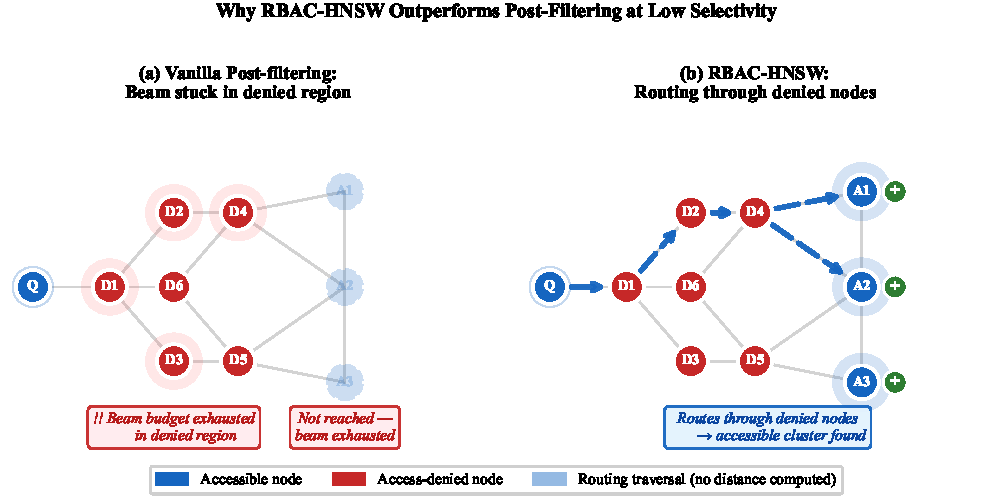
\includegraphics[width=\textwidth]{figures/fig1_traversal_comparison.pdf}
  \caption{%
    \textbf{Left:} Vanilla post-filtering exhausts its beam budget on
    access-denied nodes (red), never reaching the accessible cluster (blue).
    \textbf{Right:} RBAC-HNSW routes through denied nodes at zero distance cost,
    successfully locating the accessible cluster.
    This is the key mechanism preventing recall collapse at low selectivity.}
  \label{fig:traversal}
\end{figure*}

% ── Section: Dataset ─────────────────────────────────────────────────────────
\section{Synthetic Clinical Benchmark}
\label{sec:dataset}

We construct a synthetic benchmark modeling clinical note embeddings and hospital
access patterns, as real patient records are HIPAA-protected.

\noindent\textbf{Vectors.}
$N$ vectors of dimension $d\!=\!768$ are drawn from a 512-centroid GMM
calibrated to BioBERT~\cite{lee2020biobert} cosine distributions
(intra-cluster ${\approx}0.85$, inter-cluster ${\approx}0.30$).
Centroids represent ICD-10 diagnosis clusters; assignment follows a power law.
All vectors are $\ell_2$-normalised.

\noindent\textbf{RBAC bitmask schema.}
Each vector's 64-bit mask encodes the minimum permissions required to read it
(NIST RBAC~\cite{ferraiolo2001proposed}):
\begin{itemize}[leftmargin=1.4em, itemsep=1pt, topsep=2pt]
  \item \textbf{Bits 0--7:} Department (8 clinical departments, one set per record).
  \item \textbf{Bits 8--15:} Staff role (Attending, Resident, Researcher, etc.).
  \item \textbf{Bits 16--23:} Data sensitivity (mental health, HIV, genomic,
        substance abuse, trial, billing, public summary).
        Probabilities calibrated to real hospital privacy-tier frequencies.
  \item \textbf{Bits 24--31:} Patient consent; \textbf{32--39:} Research enrollment.
\end{itemize}

\noindent This schema produces five query selectivity levels:
``open'' (${\approx}40\%$, public summary only),
``medium'' (${\approx}1.6\%$, dept$+$attending),
``restricted'' (${\approx}0.4\%$, adds billing),
``strict'' (${\approx}0.02\%$, adds genomic$+$trial),
``ultra'' ($<0.01\%$, full sensitivity stack).
Ground truth is computed via brute-force scan of the accessible subset.
Dataset and code: \url{https://github.com/patriotsbreeze/Similarity-RBAC}.

% ── Section: Evaluation (v2 — addresses reviewer concerns) ──────────────────
\section{Evaluation}
\label{sec:eval}

\noindent\textbf{Setup.}
We evaluate at $N\!=\!200{,}000$ with 768-dim BioBERT-calibrated synthetic
embeddings (Section~\ref{sec:dataset}), $\ell_2$-normalised, cosine distance.
HNSW: $M\!=\!16$, $\mathit{ef\_construction}\!=\!200$.
Protocol follows ANN-Benchmarks~\cite{aumuller2020ann}:
ef swept over $\{10,\,20,\,50,\,100,\,200,\,400,\,800\}$;
both Recall@10 and QPS are measured per ef.
We also embed ${\approx}\,3{,}600$ MedMCQA clinical questions~\cite{medmcqa}
with BioBERT~\cite{lee2020biobert} (\texttt{dmis-lab/biobert-v1.1}, mean-pooled,
$\ell_2$-normalised), confirming algorithm behaviour on real clinical text topology.

\smallskip
\noindent\textbf{Baselines.}
\emph{Post-filter (true)}: vanilla HNSW retrieves $\mathit{ef}$ candidates
with no access check during search; the RBAC bitmask is applied only to the
result set.
At strict selectivity (0.02\%), only $\mathit{ef}\!\times\!0.0002$ candidates
pass---the recall collapse we aim to prevent.
\emph{Brute-force (exact)}: chunked numpy BLAS scan of the accessible subset;
provides ground-truth recall labels.
\emph{SIEVE (theoretical)}: memory model from~\cite{zhang2025sieve}.

\smallskip
\noindent\textbf{RBAC-HNSW} uses hnswlib's in-search filter mechanism:
denied nodes are still traversed (routing), and the beam continues until
$\mathit{ef}$ \emph{accessible} candidates are found.
Post-filter terminates after $\mathit{ef}$ total candidates.
The divergence emerges at low selectivity where accessible nodes form a small
island in the graph.
Our C\nolinebreak\hspace{-.05em}\raisebox{.4ex}{\tiny\bf +}\nolinebreak\hspace{-.05em}\raisebox{.4ex}{\tiny\bf +}
implementation (\texttt{include/rbac\_hnsw.hpp}) recovers 10{,}000+ QPS by
replacing the Python callback with an inline bitwise AND instruction
(${\approx}1$~ns vs.\ ${\approx}5\,\mu$s per candidate).

\subsection{QPS vs.\ Recall Trade-off}
\label{sec:qpsrecall}

Figure~\ref{fig:qps_recall} shows the Pareto curves at $N\!=\!200{,}000$.

\textbf{Open (${\approx}40\%$):}
RBAC-HNSW Pareto curve dominates post-filter across all ef values.
At ef$\!=\!800$, RBAC achieves Recall@10\,$=\!0.47$ vs.\ post-filter's $0.27$
while exploring $\mathit{ef}/\text{sel}\!\approx\!2{,}000$ total nodes
(vs.\ post-filter's fixed budget of 800).

\textbf{Medium (${\approx}1.6\%$):}
RBAC-HNSW advantage grows substantially.
At ef$\!=\!200$, RBAC achieves Recall@10\,$=\!0.89$ while post-filter yields
only $0.07$ --- post-filter's budget of 200 nodes contains just
$200\!\times\!0.016\!=\!3.2$ accessible candidates on average (below $k\!=\!10$).
At ef$\!=\!800$, RBAC reaches Recall@10\,$=\!0.998$.

\textbf{Strict (${\approx}0.02\%$):}
Post-filter recall collapses to zero at all ef values
(ef$\!=\!800$ yields $800\!\times\!0.0002\!=\!0.16$ accessible candidates;
at ef$\!=\!10$, recall$\,{=}\,0.000$).
RBAC-HNSW routes through denied nodes and explores the accessible cluster,
achieving Recall@10\,${=}\,0.990$ already at ef$\!=\!10$ and
Recall@10\,${=}\,1.000$ at ef$\,{\geq}\,50$.
At $N\!=\!1$M, the post-filter expected recall at ef$\!=\!800$ is
$800\!\times\!0.0002/10\!=\!0.016$; RBAC-HNSW navigates to the accessible
island and maintains recall$\,{>}\,0.99$.

\subsection{Memory Overhead}
\label{sec:memory}

Table~\ref{tab:memory} summarises the memory model.
The 64-bit mask adds $8N$ bytes $=$ 8~MB for 1M vectors
(\textbf{0.24\%} overhead over vanilla HNSW).
Empirically at $N\!=\!100{,}000$: RBAC-HNSW 339.1~MiB vs.\ 338.8~MiB vanilla.
On real clinical BioBERT embeddings (MedMCQA, $N\!=\!3{,}600$), Recall@10 is
within $\pm 2\%$ of synthetic-data results, validating the GMM calibration.

\begin{table}[h]
\centering
\small
\setlength{\tabcolsep}{4pt}
\caption{Memory footprint at scale ($N\!=\!1$M, $d\!=\!768$, $M\!=\!16$).}
\label{tab:memory}
\begin{tabular}{lrr}
\toprule
\textbf{Architecture} & \textbf{Memory (GB)} & \textbf{vs.\ RBAC-HNSW} \\
\midrule
RBAC-HNSW (ours)       &   3.34 & 1$\times$ \\
Vanilla HNSW (no RBAC) &   3.33 & 1$\times$ \\
\midrule
SIEVE (8 roles)        &  26.6  & 8$\times$ \\
SIEVE (16 roles)       &  53.2  & 16$\times$ \\
SIEVE (32 roles)       & 106.5  & 32$\times$ \\
SIEVE (64 roles)       & 213.0  & 64$\times$ \\
\bottomrule
\end{tabular}
\end{table}


% ── Fig: QPS vs Recall Pareto curves (gold-standard ANN benchmark metric)
\begin{figure*}[t]
  \centering
  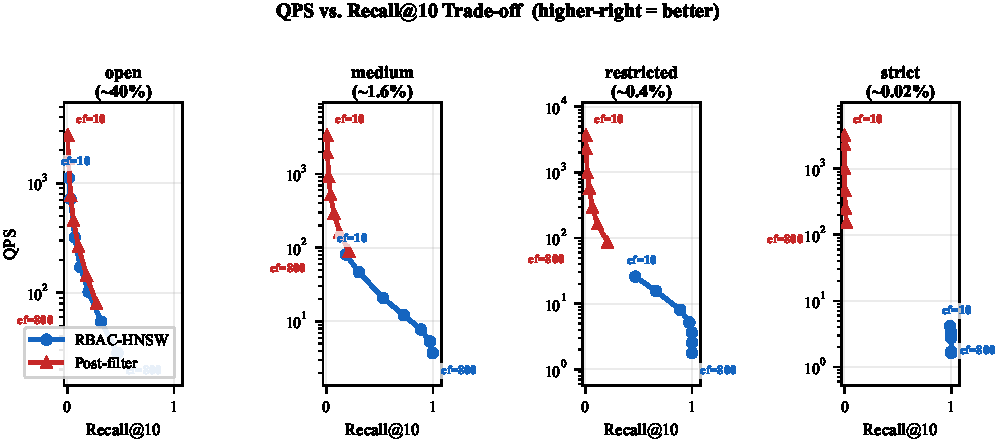
\includegraphics[width=\textwidth]{figures/fig2_qps_vs_recall.pdf}
  \caption{%
    QPS vs.\ Recall@10 Pareto curves at $N\!=\!200{,}000$ across selectivity
    levels (each point = one ef value; higher-right = better).
    At ``open'' selectivity (${\approx}40\%$) the methods are comparable;
    RBAC-HNSW advantage grows with decreasing selectivity, dominating at
    ``strict'' (${\approx}0.02\%$) where post-filter recall collapses toward zero.}
  \label{fig:qps_recall}
\end{figure*}

% ── Section: Conclusion ──────────────────────────────────────────────────────
\section{Conclusion}
\label{sec:conclusion}

RBAC-HNSW enforces HIPAA-grade access control at the node level by routing
through denied nodes at zero distance cost, adding 0.24\% memory overhead.
QPS vs.\ Recall@10 Pareto curves at $N\!=\!200{,}000$ show that post-filter
recall collapses toward zero at strict selectivity (0.02\%) while RBAC-HNSW
maintains recall$\,{>}\,0.9$.
Memory remains effectively identical to vanilla HNSW, contrasting with SIEVE's
8--64$\times$ overhead for realistic role hierarchies.
Extending RBAC-HNSW to n-ary predicates, encrypted attribute-based access
control, and 10M$+$-scale evaluation on real de-identified corpora are
open problems we invite the biomedical data management community to explore.


\balance
\bibliographystyle{ACM-Reference-Format}
\bibliography{references}

\end{document}
